% NOTE FOR AUTHORS:
% The numerical results below are from the reproducible GBM-based analysis in
% outputs/real_data_analysis. The Parametric TI uses the same boosted mean
% estimator, a global honest residual standard deviation, and a normal/chi-square
% tolerance factor. Re-run the table if the manuscript's original Parametric TI
% implementation differs.

\section{Real Data Applications}
\label{sec:real-data}

We evaluate the proposed methods on three real regression datasets chosen to
represent distinct distributional regimes: heterogeneous wages, a continuous
materials-science outcome, and semicontinuous medical expenditure. For each
dataset, we use 20 repeated random splits, allocating approximately one third of
the observations to training, calibration, and held-out evaluation. The mean,
scale, and conditional-quantile functions are estimated using gradient boosting
with a common set of tuning parameters. We set the target content to
\(C=0.90\) and the confidence level to \(1-\alpha=0.95\).

Because the conditional response distributions are unknown, we report held-out
empirical content, interval width, and the fraction of splits for which the
held-out content is at least \(C\). We refer to the last quantity as the
\emph{empirical split-success rate}. It is a finite-evaluation-sample diagnostic
and should not be interpreted as a direct estimate of the theoretical
conditional PAC guarantee or its outer probability. For CPS and MEPS, the
analysis targets the unweighted public-use sample distribution; incorporating
the complex survey designs and population weights is outside the scope of this
illustration.

\subsection{CPS Hourly Wage}

We first consider the 2012 Current Population Survey wage data. The sample
contains \(29{,}217\) observations, and the response is hourly wage. The
covariates describe sex, marital status, education, region, and labor-market
experience. Following the model specification used in the distributional
conformal prediction application, we include all two-way interactions among the
15 base covariates, yielding 100 nonconstant predictors. The methods are fitted
to log hourly wage, and the interval endpoints are transformed back to dollars
per hour.

All four methods attain empirical content above \(C=0.90\) in every split.
The average contents of SR--TI, ASR--TI, and CQR--TI are \(0.915\), \(0.915\),
and \(0.914\), respectively, compared with \(0.936\) for the Parametric TI.
CQR--TI has the smallest mean width, \(36.32\), while the Parametric TI has the
smallest 90th-percentile width, \(59.66\). Thus, in this application the
PAC-calibrated methods attain the target without a width penalty relative to
the parametric benchmark.

\subsection{Superconducting Critical Temperature}

The second dataset contains \(21{,}263\) superconducting materials represented
by 81 physicochemical summary features. The response is the critical
temperature in Kelvin, which is analyzed on its original scale. This dataset
provides a large-sample continuous-response example with pronounced variation
in conditional scale.

The three PAC-calibrated methods have nearly identical average empirical content
of \(0.917\), and all attain content at least \(0.90\) in every split. The
Parametric TI has average content \(0.907\), but its split-success rate is only
\(0.80\). Among the methods with split-success rate one, ASR--TI has the
smallest mean and 90th-percentile widths, \(42.57\) and \(78.58\),
respectively. The difference between average content and split success for the
Parametric TI illustrates why an outer-sample diagnostic is informative even
when the average held-out content is above the target.

\subsection{MEPS Medical Expenditure}

The third application uses Panel 21 of the 2016 Medical Expenditure Panel Survey
(MEPS). After applying the cohort and covariate preprocessing used in the public
CQR benchmark code, the analysis contains \(15{,}656\) individuals and 138
predictors. The response is annual total medical expenditure from the official
MEPS public-use file. Expenditure is zero for \(18.2\%\) of the observations and
has a pronounced right tail: its median is \(676.5\) dollars and its 99th
percentile is \(54{,}476.8\) dollars. We fit the methods to
\(\log(1+Y)\) and transform the interval endpoints back to dollars.

The Parametric TI undercovers, with average content \(0.884\) and a
split-success rate of \(0.05\). In contrast, SR--TI, ASR--TI, and CQR--TI have
average contents \(0.920\), \(0.921\), and \(0.920\), respectively, and attain
the target in all 20 splits. Asymmetric tail scaling reduces the mean width from
\(80{,}804\) for SR--TI to \(56{,}142\) for ASR--TI, a reduction of
approximately \(30.5\%\). CQR--TI is substantially shorter, with mean width
\(13{,}664\), reflecting its ability to adapt the lower and upper endpoints
separately to the zero mass and long upper tail. Because this response has a
point mass at zero, we view MEPS as a stress test of the finite-sample marginal
PAC layer rather than as an illustration of the continuous location--scale
conditions used for the conditional SR--TI result.

\begin{table}[H]
\centering
\caption{Real-data empirical content and interval width over 20 repeated random
splits. Split success is the fraction of splits for which held-out empirical
content is at least \(C=0.90\).}
\label{tab:real-data-summary}
\small
\begin{tabular}{llcccc}
\toprule
Dataset & Method & Content & Split success & Mean width & Q90 width \\
\midrule
CPS & SR--TI          & 0.915 & 1.00 & 37.18 & 63.17 \\
CPS & ASR--TI         & 0.915 & 1.00 & 37.68 & 64.13 \\
CPS & CQR--TI         & 0.914 & 1.00 & \textbf{36.32} & 60.06 \\
CPS & Parametric TI   & 0.936 & 1.00 & 39.77 & \textbf{59.66} \\
\midrule
Supercond. & SR--TI        & 0.917 & 1.00 & 42.61 & 78.61 \\
Supercond. & ASR--TI       & 0.917 & 1.00 & \textbf{42.57} & \textbf{78.58} \\
Supercond. & CQR--TI       & 0.917 & 1.00 & 45.98 & 79.98 \\
Supercond. & Parametric TI & 0.907 & 0.80 & 39.41 & 46.58 \\
\midrule
MEPS expenditure & SR--TI        & 0.920 & 1.00 & 80{,}804 & 179{,}317 \\
MEPS expenditure & ASR--TI       & 0.921 & 1.00 & 56{,}142 & 125{,}895 \\
MEPS expenditure & CQR--TI       & 0.920 & 1.00 & \textbf{13{,}664} & \textbf{29{,}986} \\
MEPS expenditure & Parametric TI & 0.884 & 0.05 & 113{,}044 & 313{,}210 \\
\bottomrule
\end{tabular}

\vspace{0.25em}
\begin{flushleft}
\footnotesize
Widths are reported on the original response scale: dollars per hour for CPS,
Kelvin for superconductivity, and dollars for MEPS. Bold entries indicate the
smallest width among methods attaining empirical content at least \(C\) in all
20 splits, within each dataset.
\end{flushleft}
\end{table}

\subsection{Conditional Diagnostics and Score Pivotality}

To assess the mechanism underlying the conditional interpretation, we partition
each held-out sample into quintiles of the fitted scale and report empirical
content within each quintile. We also compare each quintile-specific score CDF
with the marginal held-out score CDF using the Kolmogorov--Smirnov distance.
These calculations are descriptive diagnostics rather than tests of the
asymptotic pivotality assumption.

The scale-stratified results separate target-level behavior from full score-CDF
stability. For CPS, the CQR--TI content ranges from \(0.909\) to \(0.916\)
across scale quintiles, whereas SR--TI and ASR--TI range from approximately
\(0.878\) to \(0.947\). For superconductivity, the Parametric TI deteriorates
sharply in the highest-scale quintiles. The residual-based methods reduce this
failure, although undercoverage remains in the lowest fitted-scale quintile.
For MEPS, CQR--TI is the most stable at the target level, with quintile-specific
content between \(0.911\) and \(0.936\).

\begin{figure}[H]
\centering
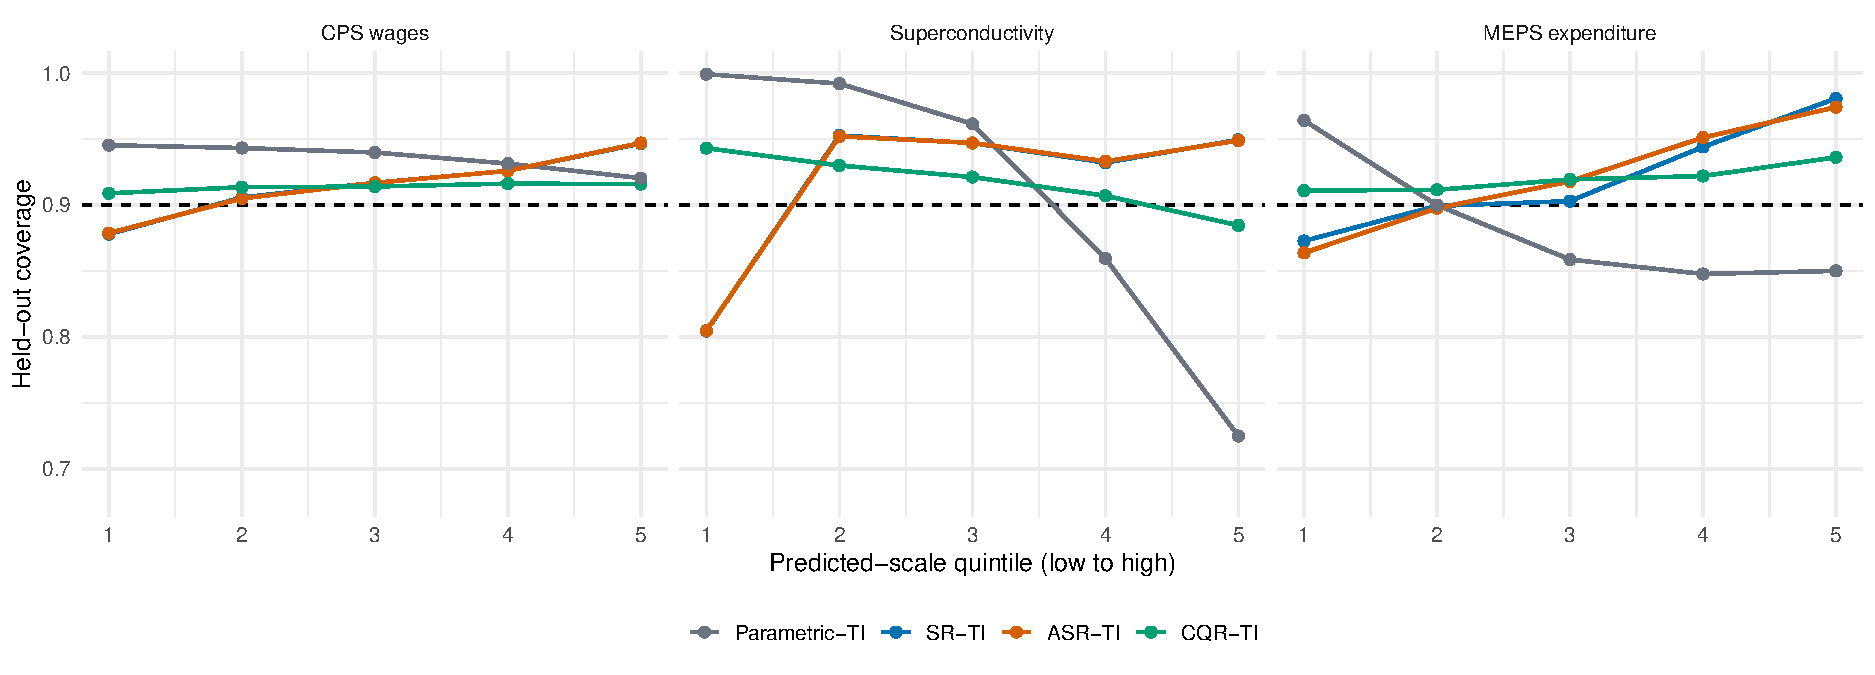
\includegraphics[width=\textwidth]{figures/coverage_by_predicted_scale.pdf}
\caption{Held-out empirical content across quintiles of the fitted conditional
scale. The dashed horizontal line denotes the target content \(C=0.90\).
Values are averaged over 20 random splits.}
\label{fig:real-data-scale-coverage}
\end{figure}

The full-CDF diagnostic gives a complementary ordering. The 90th percentile of
the empirical KS discrepancy is \(0.121\), \(0.118\), and \(0.378\) for
SR--TI, ASR--TI, and CQR--TI, respectively, on the superconductivity data.
The corresponding values are \(0.090\), \(0.090\), and \(0.115\) for CPS and
\(0.101\), \(0.096\), and \(0.170\) for MEPS. Thus, the standardized residual
scores are substantially closer to full distributional pivotality, especially
for superconductivity, even though CQR--TI can have more stable coverage at the
single target level. This pattern is consistent with the theoretical
distinction between full score pivotality, which is a sufficient transfer
condition, and alignment of the relevant conditional score quantile, which may
be enough for a fixed content level.

\begin{figure}[H]
\centering
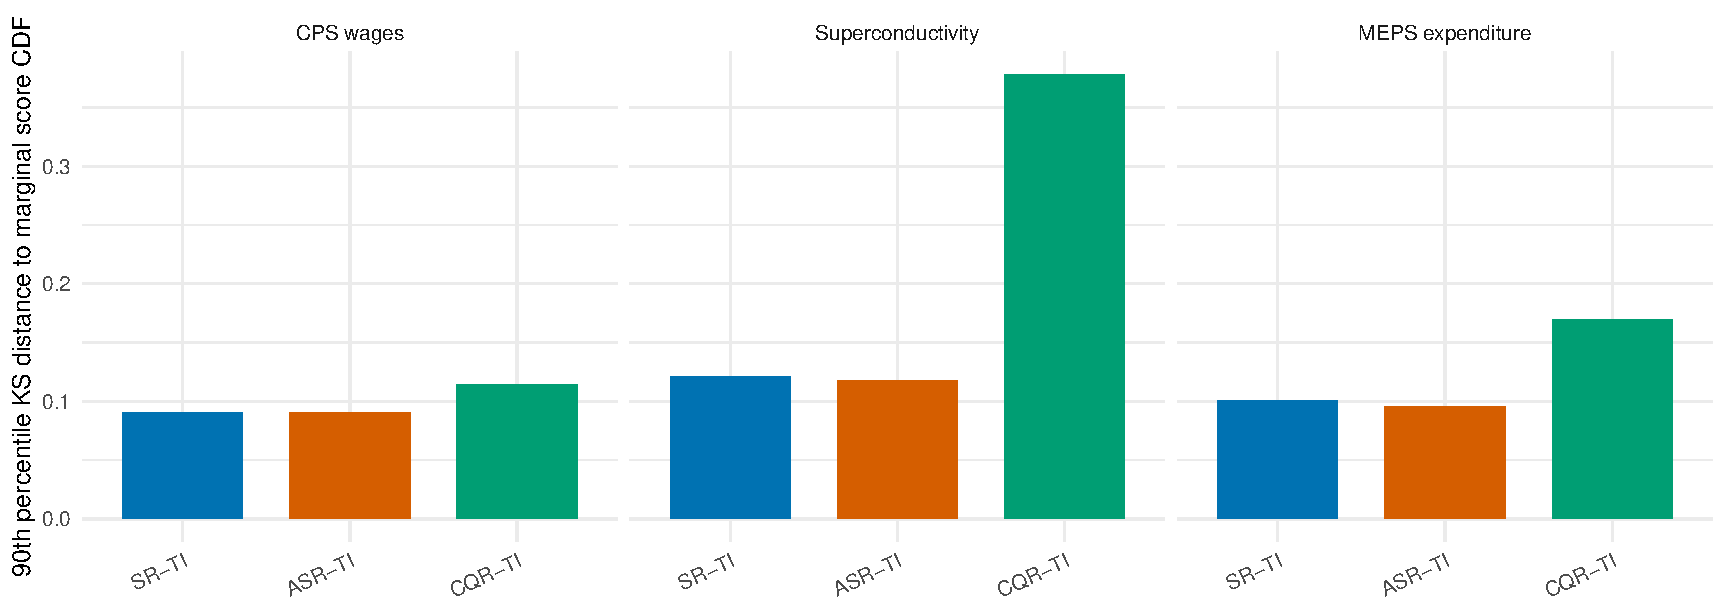
\includegraphics[width=\textwidth]{figures/score_pivotality.pdf}
\caption{Empirical score-pivotality diagnostic. Each bar is the 90th percentile,
over scale quintiles and repeated splits, of the KS distance between a
quintile-specific score CDF and the marginal held-out score CDF. Smaller values
indicate greater covariate stability of the fitted score distribution.}
\label{fig:real-data-score-pivotality}
\end{figure}

\paragraph{Takeaway.}
Across markedly different response distributions, the common
Hoeffding-adjusted calibration yields reliable marginal empirical content, but
efficiency and conditional stability remain score-dependent. CPS favors the
quantile-adaptive interval, superconductivity most clearly exhibits
residual-score pivotality, and MEPS demonstrates the value of asymmetric,
quantile-specific adaptation to a zero mass and a long upper tail.
